\documentclass[ChapterTOCs,krantz2]{krantz} % Use krantz2 for 7" x 10" trim size

\usepackage[utf8]{inputenc}
\usepackage{graphicx}
\usepackage{subfigure}
\usepackage{epigraph}
%-----------------------------------------------------------------------------
% Special-purpose color definitions (dark enough to print OK in black and white)
\usepackage{color}
\usepackage{amsthm}

% A few colors to replace the defaults for certain link types
\definecolor{orange}{cmyk}{0,0.4,0.8,0.2}
\definecolor{darkorange}{rgb}{.71,0.21,0.01}
\definecolor{darkgreen}{rgb}{.12,.54,.11}

%-----------------------------------------------------------------------------
% The hyperref package gives us a pdf with properly built
% internal navigation ('pdf bookmarks' for the table of contents,
% internal cross-reference links, web links for URLs, etc.)
%\usepackage{hyperref}

\usepackage{url}

%% Define a new 'leo' style for the package that will use a smaller font.
\makeatletter
\def\url@leostyle{%
  \@ifundefined{selectfont}{\def\UrlFont{\sf}}{\def\UrlFont{\small\ttfamily}}}
\makeatother
%% Now actually use the newly defined style.
\urlstyle{leo}

%\newcommand{\asterism}{{ \footnotesize \smash{% 
%    \raisebox{-.2ex}{% 
%      \setlength{\tabcolsep}{0.5pt}%
%      \begin{tabular}{@{}cc@{}}% 
%  \multicolumn2c*\\[-1.5ex] *&*% 
%\end{tabular}}}}}

\newcommand{\parasep}{\begin{center}*\hspace{6em}*\hspace{6em}*\end{center}}

\newcommand*{\threesim}{%
 \mathrel{\vcenter{\offinterlineskip
  \hbox{$\sim$}\vskip-.35ex\hbox{$\sim$}\vskip-.35ex\hbox{$\sim$}}}}

\newcommand{\asterism}{\smash{%
  \raisebox{-.5ex}{%
    \setlength{\tabcolsep}{-.5pt}%
    \begin{tabular}{@{}cc@{}%
  \multicolumn2c*\\[-2ex]*&*%
\end{tabular}}}}}

\theoremstyle{definition}
\newtheorem{practice}{Practice}

%-----------------------------------------------------------------------------
%
% Commands for annotating the docs with fixme and inter-author notes.  See
% below for how to disable these.
%
% Define a \fixme command to mark visually things needing fixing in the draft,
% as well as similar commands for each author to leave initialed special
% comments in the document.
% For final printing or to simply disable these bright warnings, copy
% (there's a target macros_off' in the makefile that does this) the file
% macros_off.tex to macros.tex
\usepackage{amssymb}

\newcommand{\fix}[1] { \textcolor{red} {
{\fbox{ {\bf Fix:} \ensuremath{\blacktriangleright }} {\bf #1}
\fbox{\ensuremath{\blacktriangleleft} } } } }

% And similarly, one (less jarring, with fewer symbols and no boldface) command
% for each one of us to leave comments in the main text.
\newcommand{\fperez}[1] { \textcolor{blue} {
\ensuremath{\blacklozenge} {\bf fperez:}  {#1}
\ensuremath{\blacklozenge} } }

\newcommand{\jarrod}[1] { \textcolor{darkgreen} {
\ensuremath{\bigstar} {\bf jarrod:}  {#1}
\ensuremath{\bigstar} } }

\newcommand{\mref}[1] { \textcolor{darkorange} {
\ensuremath{\blacksquare} {\bf missing ref:}  {#1}
\ensuremath{\blacksquare} } }

%% Uncomment these to turn all the special marker commands off
%\renewcommand{\fix}[1]{}
%\renewcommand{\fperez}[1]{}
%\renewcommand{\jarrod}[1]{}
%\renewcommand{\mref}[1]{}

\begin{document}

\title{Implementing Reproducible Research}
\author{Dummy author}
\chapter*{Dummy chapter needed for the \textbackslash chapterauthor command to work later}

\mainmatter

\chapterauthor{K. Jarrod Millman}{Division of Biostatistics\\
School of Public Health\\
University of California, Berkeley}
\chapterauthor{Fernando Pérez}{Henry H. Wheeler Jr. Brain Imaging Center\\
Helen Wills Neuroscience Institute\\
University of California, Berkeley\\
\\
\begin{flushright}
Dedicated to the memory of John~D.~Hunter~III, 1968-2012.
\end{flushright}}

\chapter{Developing open source scientific practice}

\section{Introduction}\label{intro}

Computational tools are at the core of modern research. In addition
to experiment and theory, the notions of simulation and data-intensive
discovery have emerged as third and fourth pillars of science \cite{4th-paradigm}.
Today, even theory and experiment are computational, as virtually
all experimental work requires computing (whether in data collection,
pre-processing or analysis) and most theoretical work requires symbolic
and numerical computing to develop and refine models. Scanning the pages
of any major scientific journal, one is hard-pressed to find a publication
in any discipline that does not depend on computing for its findings.

And yet, for all its importance, computing is often treated as an
afterthought both in the training of new scientists and in the conduct of
everyday research. Most working scientists have witnessed how computing is
treated as a task of secondary importance that students and postdocs learn
``on the go'' with little training to ensure that results are trustworthy,
comprehensible and ultimately a secure foundation for reproducible outcomes.
Software and data are stored with poor organization, documentation and tests.
A patchwork of software tools is used with limited attention paid to
capturing the complex workflows that emerge, and the evolution of code is
often not tracked over time, making it difficult to understand how a result
was obtained. Finally, many of the software packages used by scientists in
research are proprietary and closed-source, preventing the community from
having a complete understanding of the final scientific results.

\ldots

In §~\ref{sec:background}, we describe:

why we had the initial meeting

the basic idea:

* shared scientific codes (scipy)

* shared domain specific libraries (nipy)

* lab-specific development branches

In §~\ref{sec:practice} 

In §~\ref{sec:collaboration} by

In §~\ref{sec:communication} by

%In the next section, we share lessons we've learned from our participation in
%several open source development projects and describe how these lessons can be
%applied to scientific practice.  In the following section, we present a
%comprehensive view of the role computing plays in the life-cycle of scientific
%investigation.  In addition to surveying the standard approaches, this section
%ends with a detailed overview of the open source IPython project
%\cite{PER-GRA:2007}, which is a single software tool capable of spanning the
%entire life-cycle of computational research.  Finally, we conclude with a brief
%discussion of how we see the culture changing and the need for reviewing our
%current incentive models and the training of new scientists.


\section{\label{sec:background}Background}

We first describe what we believe to be the typical tools and approaches that
most working scientists use for each of these phases today, in particular
considering their impact on the reproducibility of the final outcomes. 

For \textbf{individual work}, researchers use various interactive
computing environments: Microsoft Excel, Matlab, Mathematica\textregistered,
Sage \cite{sage}, and more specialized systems like R, SPSS, SAS, and STATA for
statistics. These environments combine interactive, high-level programming
languages with a rich set of numerical and visualization libraries. The impact
of these environments cannot be overstated; they are used almost universally by
researchers for rapid prototyping, interactive exploration and data analysis,
and visualization. However, these environments have a number of limitations:
(a) some of them are proprietary and/or expensive (Excel, Matlab, Mathematica),
(b) most (except for Sage) are focused on coding in a single, relatively slow,
programming language and (c) most (except for Sage and Mathematica) do not have
a document format that is rich, i.e., that can include text, equations, images,
and video in addition to source code. While the use of proprietary tools is not
a problem \emph{per se} and may be a good solution in industry, it is a barrier
to scientific collaboration and to the construction of a common scientific
heritage where anyone can validate the work of others and build upon it.
Scientists can not share work unless all colleagues can purchase the same
package and students are forced to work with black boxes they are legally
prevented from inspecting (spectacularly defeating the very essence of
scientific inquiry). Furthermore, because of their limitations in performance
and handling large, complex code bases, these tools are mostly used for
prototyping: researchers eventually have to switch tools for building
production systems.

For \textbf{collaboration}, researchers tend to use a mix of email, version
control systems and shared network folders (Dropbox, etc.).  Version control
systems (Git, SVN, CVS, etc.) are critically important in making research
collaborative and reproducible. They allow groups to work collaboratively on
documents and track how they evolve over time. Ideally, all aspects of
computational research would be hosted on publicly available version control
repositories, such GitHub or Google Code. Unfortunately, an all-too common
approach is still for researchers to email documents to each other with ad-hoc
naming conventions that effectively provide a poor man's version control (and
are the source of endless confusion and frequent mistakes). This form of
collaboration makes it nearly impossible to track the development of a large
project and establish reproducible and testable workflows.  While a small group
can make this work by brute effort, this approach most certainly does not scale
beyond a few collaborators, as painfully experienced by anyone who has
participated in the madness of a flurry of email attachments with oddly-named
files such as {\tt paper-final-v2-REALLY-FINAL-john-oct9.doc}.

For \textbf{publications} and \textbf{education}, researchers use tools such as
\LaTeX, Google Docs or Microsoft Word/PowerPoint.  The most important attribute
of these tools in this context is that, \LaTeX{} excepted, they integrate
poorly with version control systems and are ill-suited for workflow automation.
Digital artifacts (code, data and visualizations) are often manually pasted
into these documents, which easily leads to a divergence between the
computational outcomes and the published version.  Managing this requires
manual updating, something that is error-prone and easy to forget.

From this perspective, we now draw a few lessons:

\begin{enumerate}[(a)]

\item The common approach and tools used today introduces sharp gaps between
  the stages of this workflow.  This forces researchers to switch tools at each
  stage, which in turn makes it difficult to move fluidly back and forth.
  Driven by the pressure to publish, people will then naturally charge
  \emph{forward}, pressing on to assemble results in the chase for an accepted
  manuscript but rarely going back to question assumptions, replicate earlier
  experiments with updated versions of code or parameter tweaks, etc.  Because
  reproducing results effectively requires going \emph{back} to the
  beginning of the pipeline, a workflow that from the onset makes this
  inherently difficult will likely result in outcomes that nobody, not even the
  original authors, can reliably reproduce.

  The pressure to publish in today's world encourages all scientists to charge
  forward chasing the goal of an accepted manuscript, but the very term
  ``reproducibility'' implies repetition and thus a requirement to also move
  \emph{back} to retrace one's steps, question or change assumptions and move
  forward again.

\item A key element of the problem is the disconnect that exists between what
  we view as ``final outcomes'' of the scientific effort (papers and
  presentations that contain artifacts such as figures, tables and other
  outcomes of the computation) and the pipeline that feeds these outcomes.
  Because most workflows involve a manual transfer of information (often with
  unrecorded manual changes along the way), the chances that these final
  outcomes do not match what the computational pipeline actually produces at any
  given time are high.

\item The problems listed above are \emph{both} technical and social.  While we
  focus somewhat on the tools aspect, it is critical to understand that at the
  end of the day, only when researchers make a conscious decision to adopt
  improved work habits will we see substantial improvements on this problem.
  Obviously higher-quality tools will make it easier and more appealing to
  adopt such changes, but other factors are also at play, from the natural
  inertia of ingrained habits to the external pressures applied by the
  incentive models of modern research.
\end{enumerate}

In summary, if we want to ensure that any computational research is truly
reproducible, we need to consider this entire life-cycle in an integral way and
from the beginning of a research project.  Asking about reproducibility by the
time a manuscript is ready for submission to a journal is simply too late: this
problem must be tackled from the start, not as an afterthought tacked-on at
publication time.  We must therefore look for approaches that allow researchers
to fluidly move back and forth between the above stages and that integrate
naturally into their everyday practices of research, collaboration and
publishing, so that we can make simultaneous progress on the technical and
social aspects of this issue.


Scientists as developers

Reasons

\begin{itemize}
\item  developing state-of-the-art methods
\item developing as exploration
\end{itemize}

Implications

\begin{itemize}
\item need development tools to enable
\item scientists will need to be computationally literate
\end{itemize}

Purpose:  Better Research

\begin{itemize}
\item Science becomes computing
\item Both building a hierarchical structure
\item freedom to believe differently
\end{itemize}

\subsection{Scientific Python}

Over the last decade, we've had the privilege of participating in a loose-knit
community of scientists, researchers, and engineers working to create a powerful
stack of open source tools for scientific computing written in Python.  Among
high-level open source programming languages, Python is today the leading tool
for general-purpose scientific computing (along with R for statistics),
finding wide adoption across research disciplines, education and industry and
being a core infrastructure tool at institutions such as CERN and the Hubble
Space Telescope Science Institute
\cite{millman2011python,Perez2011,ganga09,SST}.


core tools: numpy, scipy, matplotlib, and ipython

- simultaneously we've interacted heavily with researchers in
physics, psychology, neuroscience, and medicine.

- we've also talked with members of SciPy community representing
other disciplines and 

\subsection{Neuroimaging in Python}

\ldots

\subsection{Moving forward}

As research grows increasingly dependent on computing, it becomes critical
for our computational resources to be developed with the same rigor, open review
and access as the results they support.  For this reason, we actively promote:

\begin{itemize}

\item sharing of scientific software, data, and knowledge necessary for
reproducible research

\item readable, tested, validated, and documented software as the basis for
reliable scientific outcomes

\item high standards of computational literacy in the education of
mathematicians, scientists, and engineers

\item open source software developed by collaborative, meritocratic
communities

\end{itemize}

There are real issues with attempting to
naively transplant the practices of open source development directly
to computational research. The open source model ends up being one
where, in practice, the copyright and authorship of any large collaborative
project is spread among many authors, possibly thousands. While
the source control tools in use do allow for a relatively precise
provenance analysis to be performed if desired, this is rarely done
and its success is contingent on the community having followed certain
steps rigorously to ensure that attribution was correctly recorded
during development.

This is not a major issue in open source, as the rewards mechanisms
tend to be more informal and based on the overall recognition of any
one contributor in the community. Sometimes people contribute to open
source projects as part of their official work responsibilities, and
in that case a company can enact whatever policies it deems necessary;
often contributions are made by volunteers for whom an acknowledgment
in the project's credits is sufficient recognition.

In contrast, the academic world overwhelmingly weighs the authorship
of scholarly articles and conference proceedings as the main driver
of all forms of professional advancement and reward. In this system,
the pecking order of authorship matters enormously (with the many
unpleasant consequences familiar to all of us), and so does the total
number of authors in a publication. While in certain communities papers
with thousands of authors do exist (experimental high-energy physics
being the classic example), most scientists need the prominent visibility
they can achieve in a short author list. The dilution of authorship
resulting from a largely open collaborative development model
is an important issue that must be addressed.

Furthermore, the notion of a fully open development model typical
of open source projects is at odds with another aspect of the
scientific publication and reward system: the ``first
to publish'' race. Many scientists are, understandably,
leery of exposing their projects on an openly accessible website
when in their embryonic stages. The fear of being scooped by others
is real, and again we must properly address it as we consider
how to apply the lessons of open source development to the scientific
context.

In summary, we think that a few simple lessons can be learned from
the practices of the open source world which, if carefully assimilated,
can lead to substantial improvements in the state of reproducible
computational research. 

For more information, we highly recommend the recent archiv preprint
\ldots \cite{2012arXiv1210.0530A}.

\section{\label{sec:practice}Routine practice}

The practices recommended in this section are distilled from years of
experience writing and maintaining software, teaching programming courses to
students and scientists, as well as extensive interaction and discussion with a
diverse group of scientists and engineers.  Whole books have been dedicated to
best practices in software development with highly specialized tools and habits
for individual programming languages and tools.  In this short section, we
highlight the practices and tools essential to any computational work.

We begin by discussing practices and tools that should be applied to even
exploratory, individual research.  These practices are so essential to
efficient and productive use of computational resources that we routinely use
them whenever we use a computer. In the following section, we discuss how these
practices and tools naturally extend to collaborative work. 

\subsection{Version control}

Whether you are collecting data, running analyses, or writing papers,
you will inevitably need to keep track of the various versions of your work:
data is augmented and curated; code is adapted and improved; and writing is
revised and expanded.  While simply keeping the most recent version of your
work sounds like a reasonable approach, in practice, this is seldom sufficient.
There are tentative new directions, detours, and dead ends.

We've witnessed numerous researchers attempting to manage different versions of
their work using manual and laborious kludges. The most common patterns include
using \emph{ad hoc} naming schemes (e.g., \texttt{file.txt.bak},
\texttt{file.txt.1st}, etc.), emailing different versions to yourself, or using
the specialized functionality built into the tool you happen to use (e.g.,
Microsoft Word's ``Track Changes'' functionality).  While these approaches are
partial solutions to the problem, they are also cumbersome and prone to
failure.  More importantly, they are unsustainable beyond very
simple scenarios with only one or two files and do not scale to any kind of
sensible collaboration workflow.

Because tracking and managing how work evolves over time is so fundamental to
the workflow of software development, programmers have created specialized
software tools to do exactly this. These tools are called \emph{version
  control} systems. Several open source version control systems (VCS) have been
developed over the years, the most well known being CVS, SVN, Git, and
Mercurial.

While there are notable differences among these tools, they all share some
basic concepts.  You store all your project files (code,
text, figures, etc.) in a \emph{repository} (often represented on disk in a
directory hierarchy).  There are commands to add and remove files to a
repository.  When you change a file in your repository that you want to track,
you can \emph{commit} those changes with a \emph{commit message}.  The
repository and commit mechanism provide a complete historical log of the
project from inception to current state, including every change made along with
timestamps, author, comments and other metadata for each modification.

Commonly your changes may follow a simple linear progression of commits.
However it is reasonable to have a project evolve so that it does not follow a
straight route from beginning to end. For example, given the exploratory nature
of research, you may have several alternative approaches that you want to try
out. In such cases, your commits will resemble a tree with several
\emph{branches} diverging from a common base or trunk. When exploring these
alternative approaches on different branches, you may find that several
branches converge. At this point, you will \emph{merge} these
branches back together.  If the changes in each of these branches don't overlap
with one another, the VCS is capable of merging them all together in a
completely automated fashion.  When you have \emph{conflicting} changes in
different branches (e.g., edits to the same line of code), then the VCS
require manual intervention where you have to choose which of the conflicting
changes should ultimately prevail.  But in all cases, a VCS is the only
reasonable solution for managing the evolution of multiple branches of parallel
development in a set of files (whether written documents, computer code or
data).

In the design of more modern VCS such as Mercurial and Git, an important
consideration has been woven into the core of the system: built-in \emph{data
  integrity verification} via cryptographically robust fingerprinting of all
content.  The basic idea is that at every commit, the VCS computes a
``fingerprint'' of the content being committed as well as the data it depended
on\footnote{More precisely, a hash function is evaluated on the content of the
  commit and the hash of all commits it depends on, which creates a directed
  acyclic graph of hash values that signs the entire repository.  Today these
  systems employ the SHA1 hash function, but other hashes could be equally used
  if necessary}.  In this manner, at any point in time it is possible to
establish the integrity of the entire history of a repository, by recomputing
these fingerprints and comparing them against what has been stored.  By the
nature of hash functions, if even a single byte is changed in the entire
repository all subsequent hashes will be modified and the change can thus be
detected.  This key design idea is used by VCS for all kinds of internal
operations, but it also means that when a scientist gets a copy of a
repository, he or she can be confident, with near mathematical certainty, that
the entire history contained therein has not been tampered with in any way when
compared to another repository with the same hashes.  

Strong guarantees on data integrity are a necessary condition of any
reproducible workflow, and one of the reasons why we emphasize so much the
pervasive use of modern version control systems as the foundation of a
reproducible research environment.

It is important to note that VCS were developed originally for the
management of human-generated content such as computer source code or text
documents, not for the handling of large binary data that is common in science.
By virtue of their design, they tend to be somewhat inefficient if you attempt
to store all the changes in a project with many frequently changing large
binary files, and this somewhat limits their use for the tracking of all assets
in a research project.  But new efforts exist to mitigate these limitations,
such as the git-annex project\footnote{\url{http://git-annex.branchable.com}}
that uses Git for storing all metadata about large binary assets, along
with a static (configurable) storage resource external to Git for the assets
themselves.  This approach makes it possible to smoothly integrate the
management of binary data within a VCS workflow, without creating an explosion
in the size of the VCS storage area.

In summary, the use of version control should be seen as a ``background
technology''; in our case its use is so routine that we use it for everything:
writing grants and papers, teaching materials, homework, slides for talks, etc.
This leads us to suggest our first ``recipe'' in terms of best practices:

\begin{practice}
  Pervasive version control: research codes, manuscripts and data analysis
  projects should be developed, from the beginning, \emph{always} using version
  control systems that track the actual history of everyone's contributions.
\end{practice}

\subsection{Testing}

Computing is error-prone. While there is no
fool-proof way to rid computing of error, there are ways to limit and reduce
it. One of the most successful and widely used techniques involves
comprehensive testing, so that bugs (i.e., errors) are found quickly. Finding
bugs as soon as possible in the development process is extremely valuable.
Depending on the nature of the bug, it may reveal a fundamental problem with
the overall design of your code requiring months more of coding.  Even small
errors that are easily fixed may require rerunning months of analysis.
Debugging is the process of fixing bugs that you find and it can be a
painstaking ordeal. To reduce the amount of time it takes to uncover bugs and
to ease the pain of debugging your code, it is essential to adopt a rigorous
testing practice up front.%
\footnote{While testing is extremely useful
practice, we should also point out that it is often much more interesting work
than debugging.} Beware though, as E. W. Dijkstra famously observed, ``Program
testing can be used to show the presence of bugs, but never to show their
absence!'' \cite{dahl1972structured}

Testing must be performed on multiple levels. If your program takes input
either from a user or file, then it is important that the code checks that the
input is exactly what the program expects. You will also want to write
\emph{unit tests} to ensure that unitary code elements like functions, classes,
and class methods behave correctly. And finally, you will want to write
\emph{regression tests} to make sure you do not break existing functionality.
For instance, you could have a previous analysis rerun to make sure that the
program reproduces your previous results.

Testing should be done as early as possible in the development process.
Writing unit tests early in the process of implementing new functionality
forces you to think about what you want a piece of code to do, rather than how
it does it. This practice helps improves code quality by forcing you to focus
on use cases rather than getting lost in implementation details. By thinking
about the test at the outset, you can avoid finding that the code you just
wrote is a huge untestable mess. It can also improve documentation because an
example (i.e., the test case) is often better than an explanation. And if you
regularly run the test, you will quickly know when your code no longer works
for the example (something you may never notice in the case of explanatory
text). Finally, you will have more robust code as you will more quickly
isolate bugs, which makes them easier to fix.\cite{oram2010making}

%\paragraph{ {\bf Computational practice}}
%
%\setlength{\epigraphrule}{0pt}
%\setlength{\epigraphwidth}{.90\textwidth}
%\epigraph%
%{%
%  In ordinary computational practice by hand or by desk machines, it
%  is the custom to check every step of the computation and, when an
%  error is found, to localize it by a backward process starting from
%  the first point where the error is noted.
%}%
%{\textit{Cybernetics (1948)}\\ \textsc{Norbert Wiener} }
%
%Computing is now synonymous with the use of automated, electronic machines.  So
%synonymous, in fact, that is easy to forget that computing has always been part
%of scientific investigation. Of course, the types of problems amenable to
%computing by hand on paper or with early calculating machines (e.g., abacus)
%were limited. 
%
%Lessons we all were taught in our elementary mathematics classes:
%
%- show your work
%
%- need to double check answers
%
%- ease of making a mistake
%
%As automated, electronic computing machines were developed by scientists,
%those same grade school practices were standard.  Code and methods were
%openly shared and discussed, rigorous testing procedures, etc.
%

\subsection{Readability}

While writing code that is well-tested and systematically managed by a modern
VCS is important, code that you (and your colleagues) can't read is
nearly useless. Readable code is written with explanatory names, clear logical
structure, and comprehensive documentation where necessary.  There is an
extensive and growing literature (e.g., \cite{boswell2011art, Fow00,
kernighan1999practice, HT00, mcconnell2009code}) on ``stylistic'' aspects of
good programming. Because scientific papers and grant submissions have become
the currency of the scientific realm, many scientists have spent at least some time reading classics such as Strunk \&
White's \emph{Elements of Style}. Yet, even as an increasing amount of our
work is produced in lines of code, there is a paucity of scientists paying the
same attention to the elements of good programming style. The emphasis on
readability is included in this section because even when you are the only one
using or working on your code, the chance that you will need to read your own
code is high. Even when your code is widely used and shared, the chances are
that you still will be the one most frequently reading your own code.

Given the literature on the subject, written by more experienced programmers,
we will only briefly touch on self-documenting code. Self-documenting code, as
the name implies, reduces the need for external documentation by placing an
emphasis on clear, well-written code that is easy to read and understand.  In
mathematics, it is accepted practice to follow established naming conventions
(e.g., capital letters for sets and lower case letter for set elements). It is
equally expected that when making a mathematical argument, one shouldn't
arbitrarily switch from functional to relational notation.  Similarly, using
consistent and uniform naming conventions when programming should be standard
practice. Brevity in naming should be balanced against explicit and descriptive
words. For example, you might use the term \texttt{download} rather than
\texttt{get} in a function call to download a specific dataset from the
internet. Expressions are the next block to readability. While mathematical
manipulation (e.g., De Morgan's laws) can be used to great effect in making
your expressions more easily understood, it is often important to use the right
level of abstraction. Higher level programming languages (e.g., Python
and R) provide data structures (such as $n$-dimensional vectors or statistical
formulas) that enable the code to be understood at the level of the
mathematical ideas. Finally, the overall control flow of your code must be
clear and easy to follow. Finding the best control flow requires a deep
understanding of your problem and an in-depth knowledge of programming
methodology and the specifics of the language you are working in. Like good
writing, good coding is achieved through deliberate practice.

Readability in programming encompasses not just the code itself,
but also the accompanying documentation. Code comments offer much to readability,
but are sadly used to little positive effect. Inspired by the idea of
self-documenting code, we've heard programmers argue that good code doesn't
need comments. Indeed, liberally commenting your program to counter poorly
written, obscure code is poor practice. Comments that simply explain how a piece
of code works are often unhelpful. If code is so obscure to need explanation,
it is perhaps better to rewrite or refactor it. One problem with comments (as
with many types of documentation) is that it is often uncoupled with the actual
code. This means that there is no way to ensure that the two don't diverge.
And, if they diverge, it may not be obvious which is at fault.

To illustrate how comments and documentation can enhance readability of your
code, we discuss the commenting and documentation system that has been
developed by NumPy and is being used by other scientific Python projects. While
this section is specific to the tools and processes put in place in the
scientific Python community, the general ideas are more broadly applicable.

By 2007, NumPy provided the foundation layer for numerical, scientific
computing in Python. With over a decade of development effort behind it, NumPy
had evolved (with the help of numerous developers and users) to a powerful and
widely used package. However, there was a lack of good reference information
for the various functions, classes, and modules it provided. Users and
developers had access to the source code, an almost 400 page ``Guide to
NumPy'', and an active mailing list. Yet, it was clear that this level of
documentation wasn't enough. To address this, the community began a year long
effort to develop a documentation string standard. In Python, a documentation
string (or docstring) is any string in the first line in an object's (function,
class, etc.) definition. Since docstrings are embedded in the source code, they
are readily available to anyone directly viewing the source. The string is
associated with the object and can be programmatically accessed as well.  They
can be accessed from an interpreter using any object's \texttt{\_\_doc\_\_}
attribute.  Docstrings can also be accessed for autogenerating documentation.
Similar functionality exists in other programming languages such as R. And even
in language that don't include this functionality, it is common practice to
include comments at the beginning of object definitions that are used
similarly.

Given a recognized need for better documentation and documentation
functionality that we wanted to leverage, the discussion focused on what this
documentation should include. Besides the need to include information such as a
brief statement of purpose as well as input and output parameters, there were
several issues that arose with special relevance for scientific applications.
For instance, many of the algorithms had simple mathematical expressions that
weren't necessarily obvious from there implementation in Python. In these
cases, a few equations written in \LaTeX{} were immediately useful. Moreover,
in several cases, we were implementing functionality that was described in
peer-reviewed academic journals. And, finally, we could provide extremely
short examples of how to use the code. As an added benefit, Python makes it
easy to include examples in the docstrings as part of the test suite; this
improves the test coverage and helps ensure that the documentation doesn't get
out of sync with the actual code.

\subsection{Infrastructure}

For very small projects, managing everything by hand may be straightforward.
But as your research project (code, data, and text) evolves, the burden of
running your tests, building your project, and generating reports will become
overwhelming. Eventually you will need tools and procedures in place to take
care of these details for you. Even when the project is small enough that you
can manually manage things, automating these tasks can be extremely beneficial.
\cite{doar2005practical}

\begin{itemize}

\item Tests runners and continuous integration, coverage

\item Make vs IDE

\item auto-generated API documentation, NumPy documentation system \cite{SciPyProceedings_27}

\item online resources: trac, redmine, vs hosted project management like
      sourceforge, github

\end{itemize}

\section{\label{sec:collaboration}Collaboration}

Collaboration is essential to both the scientific and open source communities.
Open source developers build on one another's work just as scientists build on
each others work.  Yet the practices and tools in open source software
development are much more advanced when it comes to collaboration. Since
development communities are geographically spread and often dependent on
contributions from volunteers, there has been careful attention paid to
efficient and productive tools and processes for managing collaborations.  As
scientific practice becomes increasingly computational, it is imperative that
we learn from the collaborative practices used in the open source world.

Before discussing some of the collaboration tools and practices used in open
source development, we briefly briefly underscore the need to adopt such tools
by highlighting a few ways that the current lack of collaboration among
scientists on software tools is impeding progress. Even when researchers
release the analysis code under an open source license, it is too often the
case that they don't develop it in a collobarative, open source manner.
These analysis packages are often developed by one scientist or by researchers
in one lab. If two different packages are developed to do similar types
of analysis by two competing labs, then what package gains the widest adoption
by the community may be decided by factors other than scientific merit. For
instance, the package that is easiest to install, use, or modify will have
a much better chance of adoption. And since new algorithm implementations
are provided in competing, and often none interoperable, packages the
competition takes place at the level of software---not algorithms. Of course,
there are also purely wasted effort considerations when each lab is separately
implementing and maintaining code for all the miscellaneous aspects of
analysis software such as reading and writing data.


\subsection{Distributed version control}

Earlier we discussed how version control system (VCS) should be the foundation of a
reproducible research workflow, even for a single investigator working in
isolation.  But the true power of these systems comes into its own when
considering the need to collaborate with others.  Modern systems such as Git
and Mercurial were designed from the ground up for large-scale distributed
collaboration: Git was written by Linus Torvalds, the creator of the Linux
kernel, to coordinate its development.  The Linux kernel is arguably the
largest and most complex single open source development project today: version
3.7 of the kernel included roughly 12,000 distinct sets of changes affecting
over 1,100,000 lines of code by nearly 1,300 individual
contributors\footnote{\url{https://lwn.net/Articles/526748}}.  Git's entire
design aims to make collaboration on this scale smooth and efficient, and it
succeeds admirably at the task.  Scientists can benefit from this power as well
for any project that requires collaboration, whether it is the development of
an open source research code or the writing of a manuscript or grant proposal
with multiple authors.

Git and other tools like it are called \emph{distributed} version control
systems (DVCS) because they don't depend on a central server for their functioning,
instead maintaining the entire history of a project inside every repository.
This is in contrast to legacy systems such as CVS and SVN, that made a
distinction between the ``working copy'' that users would work on and which
contained only the most recent version of files, and a special repository
hosted on a central server that had the entire project history.  The
centralized model does enable collaboration, but it also creates a number of
problems that the distributed model addresses.  In a DVCS there is no single
point of failure, as every repository carries all the project history and
therefore serves as an automatic backup.

More importantly, a DVCS enables anyone who can \emph{clone} a repository (the
term used to indicate getting a full copy of an existing repository to start
new work off of it) to develop their own history with new commits, even if they
don't have write permission to the original source from where the repository
was cloned.  This means that once you have a clone of a repository (which could
be someone else's or yours from a different computer), you can start working on
that copy and building new history even if you are disconnected from the
original system, such as when working on a plane or train without internet
access.  If at a later stage you decide to merge your new history with the
original repository, the merge capabilities in all DVCS make this very
straightforward.

This model of cloning an existing repository, building new history in isolation
and then merging it back into a common history, is the basis for how these
systems enable a very fluid workflow for collaboration.  When the time comes to
need a merge operation, DVCS can communicate the necessary changes even
via email attachments, but the simplest way to do so is to have a special
repository\footnote{We note that this central repository does not change the
  distributed nature of the process: while it plays a special role for purposes
  of \emph{synchronization}, the central repository is otherwise completely
  symmetrical to everyone's personal copy in the information it holds, and can
  be replaced at any time in case it is lost or damaged from anyone's copy.} in
a common location that all parties have access to and where the changes are
\emph{pushed} to.  Pushing, as the term suggests, means sending the set of
changes from one repository into another; once the changes have been put into
this central repository, all parties can \emph{pull} them into their personal
copies to synchronize their states and continue working again.  So in practice,
the simplest and most common collaboration workflow with a DVCS is one where
each person has a copy they develop on, and they all connect in a star topology
to a central node where a shared copy exists that is used for synchronization.

\subsection{Code review}

In recent years, a number of web services have appeared that play the role of
this central node; the most popular of them by far is
GitHub\footnote{\url{http://github.com}}, but others such as
BitBucket\footnote{\url{https://bitbucket.org}} and
Gitorious\footnote{\url{http://gitorious.org}} play similar roles.  GitHub has
had a tremendous impact in the open source community, reaching in a few years
millions of active users and gaining rapidly popularity in scientific circles.
We can attest to the power of this platform with our own experience: the open
source IPython project (see §~\ref{IPython}) moved its development to GitHub in
early 2010 and immediately saw a rapid uptick in the pace of contributions.
The workflow for collaboration enabled by GitHub was so much smoother than all
previously available tools that many people were more willing to send
contributions, while the core team was able to review and integrate these
contributions at a much more rapid pace.

The core element of the collaborative process on GitHub is known as a
\emph{pull request}, and it is something akin to a public peer review of a set
of changes to a manuscript.  Let us illustrate how it works with a simple
example: Alice wants to contribute to IPython, a project available on github at
\url{http://github.com/ipython} but to which she does not have write access.
She can do so by getting her own personal copy of the IPython Git repository
where she makes all the changes she wants, and once she is ready to share them
with the IPython team she can publish them on her GitHub user account at
\url{http://gitub.com/alice/ipython} (presuming her GitHub user name is
\texttt{alice} for the sake of this example).  At that point, she can click on
a button to create a ``pull request'' for these changes: this contacts the
IPython developers and creates a special page on the website that summarizes
her changes as well as allowing everyone to begin a discussion about the nature
of these changes.  This discussion page allows the developers to ask Alice
questions (even making comments on specific lines of her new code), and she can
respond to these questions, update her code with new commits in order to
address any required improvements, etc.  Once the IPython developers are
satisfied with this review and discussion (which may happen immediately or may
require a lengthy back-and-forth process, depending on the nature of the
changes), they can apply the changes to the official IPython repository with a
click of a button\footnote{This is an example of a real pull request page for
  IPython that already went through the entire review process:
  \url{https://github.com/ipython/ipython/pull/1732}}.  Once the changes are
merged, they become part of the official project source and every individual
commit that was merged is credited to Alice from the time she made it while she
was working on her personal copy.  Furthermore, even closed pull requests
remain available on the website to inform future discussions, making the entire
collaboration process an open one.

This pull request process allows for a dynamic and open peer review process of
all proposed changes to a project, while everyone has access to the same
version control tools while they work.  The only special role that the official
project authors have is the ability to approve the final merging of new
changes, but otherwise everyone participates on an equal footing in terms of
access to tools.  

In our experience, this highly symmetrical structure proves to be extremely
beneficial in encouraging a very meritocratic process of contribution and
review, where there are very few points of special authority and where the
discussions can remain focused around the contribution that initiated the pull
request.  Paraphrasing how some of the GitHub employees describe the process in
public presentations: ``a pull request is a conversation that starts with
code''.  From a scientific research perspective, we should consider these ideas
in a broader context that goes beyond code: while peer review is one of the
very pillars of how the scientific community moves forward, in practice modern
scientific peer review is often an opaque, arbitrary, and limited process.  The
open, dynamic, and ongoing process of peer review enabled by the GitHub pull
request system (or the equivalent ones that exist on other similar services)
stands in sharp contrast to some of our scientific traditions, and in our
opinion our community could benefit significantly from adopting some of these
ideas in a more pervasive manner in our own review practices
\cite{10.3389/fncom.2012.00018}.

It is worth noting that by using a DVCS, authors can maintain private work
branches in the context of a publicly available project; this can be useful if
new work needs to be developed in private prior to publication and subsequent
public release. By tracking the public repository but keeping a private branch,
they can maintain exclusive access to their new work until it is published,
while continuing to develop the openly accessible code with the rest of the
scientific community. Once the code is published, since it was developed using
the same version control machinery of the public branch, the new contributions
can be seamlessly merged with the public version and their entire provenance
(including information such as time of invention and individual credit within
the lab) becomes available for inspection.  This simple observation shows how
these tools can be used to balance the sometimes valid requests for privacy
that may exist in a research environment with the desire for subsequent
disclosure and publication, without losing any of the benefits of version
control with regards to attribution and provenance tracking.

\subsection{Infrastructure redux}


- github test integration



\section{\label{sec:communication}Communication}

\setlength{\epigraphrule}{0pt}
\setlength{\epigraphwidth}{.90\textwidth}
\epigraph%
{%
Instead of imagining that our main task is to instruct a \emph{computer}
what to do, let us concentrate rather on explaining to \emph{human beings}
what we want a computer to do.
}%
{\textit{Literate programming (1984)}\\ \textsc{Donald Knuth} }

In this section, we will present a perspective on the problem of
computational research that takes a unified view of the life-cycle of research
ideas, to show how the majority of existing tools make it difficult to manage
this life-cycle in a way that naturally leads to reproducible outcomes.  We
will briefly review some of the existing prior work dating back to D. Knuth on
literate programming \cite{Knuth92} and mention current progress in that
direction mostly coming from the vibrant R community, and we will then focus on
work recently done in the scientific Python community that takes a slightly
different angle on these questions than the traditional literate programming
approach.


With the above in mind, our approach to the problem of reproducibility in
computational research will then be focused on building tools and practices
that enable researchers to naturally consider the entire cycle of research as a
continuum, and where ``doing the right thing'' is the easy and natural path
rather than the awkward and cumbersome one.  We will first briefly describe the
existing tools for literate programming as the backdrop against which we will
introduce a contrasting approach that we refer to as ``literate computing''.
We argue that this approach is a better fit to the needs of reproducibility in
computational research and will present tools that have been developed recently
in the open source community in this direction.



\subsection{Literate programming}


The concept of \emph{Literate Programming} was introduced by Donald Knuth in
the early 1980's \cite{Knuth:1983:LP} and a complete description of this
approach to computer programming can be found in his later book of the same
title \cite{Knuth92}.  Knuth's concern was the development of a better approach
to documenting computer software; he devised a process whereby programmers
would write literate source files that describe in full prose the ideas
underlying a given program, interspersed with the code fragments implementing
the actual computations.  Knuth developed tools that can process these input
files to produce two different representations: a ``tangled'' code file meant
for compilation and execution by a computer, and a ``woven'' file containing
the formatted documentation.  Knuth's original implementation, the WEB system
\cite{Knuth:1983:WSS}, was focused on producing Pascal code and \LaTeX
documentation, but this basic idea has been extended to many other programming
languages and documentation systems.  

The R community has actively embraced the ideas behind literate programming,
and a mature implementation of the concept exists for R in the Sweave system
\cite{lmucs-papers:Leisch:2002}.  Sweave is one of the central elements of the
Bioconductor system \cite{Gentleman2004, Dudoit2003} for computational biology
and bioinformatics.  As all Bioconductor packages must be accompanied by at
least one ``vignette'', a literate programming document that contains
executable code illustrating the tasks the package is meant to perform.
Vignettes can be read in PDF format, but functions exist to automatically
extract all the R code for immediate execution.  The journal Biostatistics
encourages authors to use literate programming tools such as \LaTeX and Sweave
when submitting articles they wish to be desingated reproducible \cite{Peng01072009}.

In recent years, a new entrant to the R community that is gaining rapid
adoption is the knitr package \cite{xie2012knitr}.  Knitr can be seen as a
highly evolved Sweave with a number of improvements on many fronts, but still
within the conceptual lineage of literate programming tools.  The use of
literate programming tools are gaining increasing traction in statistical
education as well.  For instance, at UC Berkeley, students taking computational
classes in both the Statistics Department and the Divison of Biostatistics are
now strongly encouraged to use \LaTeX with Sweave or \LaTeX (or R Markdown) with 
knitr.

As the above examples suggest, literate programming has been most commonly
adopted when the desired final document is intend primarily for human
consumption.  Few, if any, large software libraries are written this way.
In fact, the most prevalent use of literate programming has been among
scientists to communicate computational ideas and results to one another.
The other area where these ideas have had a big impact is in open source
software projects where tools have been developed to automatical generate
project documentation based on source files or in creating ``live''
documentation with embedded code run during document generation.\footnote{
For instance, Sphinx (http://sphinx-doc.org/) is a document generation tool
that is used for many Python projects including all the major scientific
Python packages.} 

\subsection{Literate computing}

Tools described in the previous section for literate programming are mature and
have been used to great effect to improve the quality of documentation in
scientific programs and data analysis, especially in the R community.  But they
remain firmly rooted in the original model proposed by Knuth, of authoring a
literate file that is then post-processed by various tools to produce either
documentation or executable code.  

In this section, we will contrast these with an alternate approach to the same
questions of improving the connection between code and documentation, that we
refer to as ``literate computing''.  Our choice of terminology points to the
fact that we emphasize the act of computing itself rather than the writing of
code, as all the systems we will describe are all centered around
\emph{interactive environments} where the user can enter code for immediate
execution, obtain results, and continue with more commands that produce new
results based on the previous ones.  A literate computing environment is one
that allows users not only to execute commands but also to store in a literate
document format the results of these commands along with figures and free-form
text that typically can include formatted mathematical expressions.  In
practice it can be seen as a blend of a command-line environment such as the
Unix shell with a word processor, since the resulting documents can be read
like text, but contain blocks of code that were executed by the underlying
computational system.

The earliest full-fledged implementation of these ideas is the graphical user
interface of the Mathematica \emph{Notebook} system which dates back to early
versions of Mathematica on the NeXT computer platform and took advantage of the
superior graphical capabilities of NeXT.  Today a number of other systems (both
open source and proprietary) provide similar capabilities; on the open-source
front we notably mention the Maxima \mref{maxima notebook} symbolic computing
package, the Sage \mref{sage} mathematical computing system, and the
interactive computing project IPython, on which we will focus the rest of our
discussion.

\subsection{IPython notebook}\label{IPython}

IPython\footnote{\url{http://ipython.org}} is a system for interactive and
parallel computing that has become the \emph{de facto} standard environment for
scientific computing and data analysis in the Python programming language.  It
was created by F. Pérez in in 2001 as an interactive command-line shell for
Python, and has evolved into a large collaborative open-source project with
contributions from a broad team of scientists \cite{PER-GRA:2007}.  IPython
started with the simple purpose of building a better interactive environment
for everyday computational work by a single researcher.  But as it grew into a
broader open source project, the team working on it (most of them practicing
scientists) learned many of the skills of the trade from open source software
developers.  It is precisely from this interplay between scientific research
and software development that we highlight here, as through contact with the
tools and culture of the open source world, we saw how in many respects this
community had outpaced scientists in its robust and rigorous use of
computational resources.  Through the years, we have thus led a dual life,
where the contact with this open source community continually informs and
enriches our approach to computational research and has helped us build IPython
into a better scientific tool.

In 2011, a web-based notebook was developed in IPython that connects to the
same interactive core as the original command-line shell, but does so using a
web browser as the user interface, automatically enabling either local or
remote use as the system running the web browser can be different from that
executing the code, with all communication happening over the network.
Fig.~\ref{fig:IPython-notebook} shows a typical notebook session with code,
text, mathematics and figures.

\begin{figure}
  \begin{centering}
    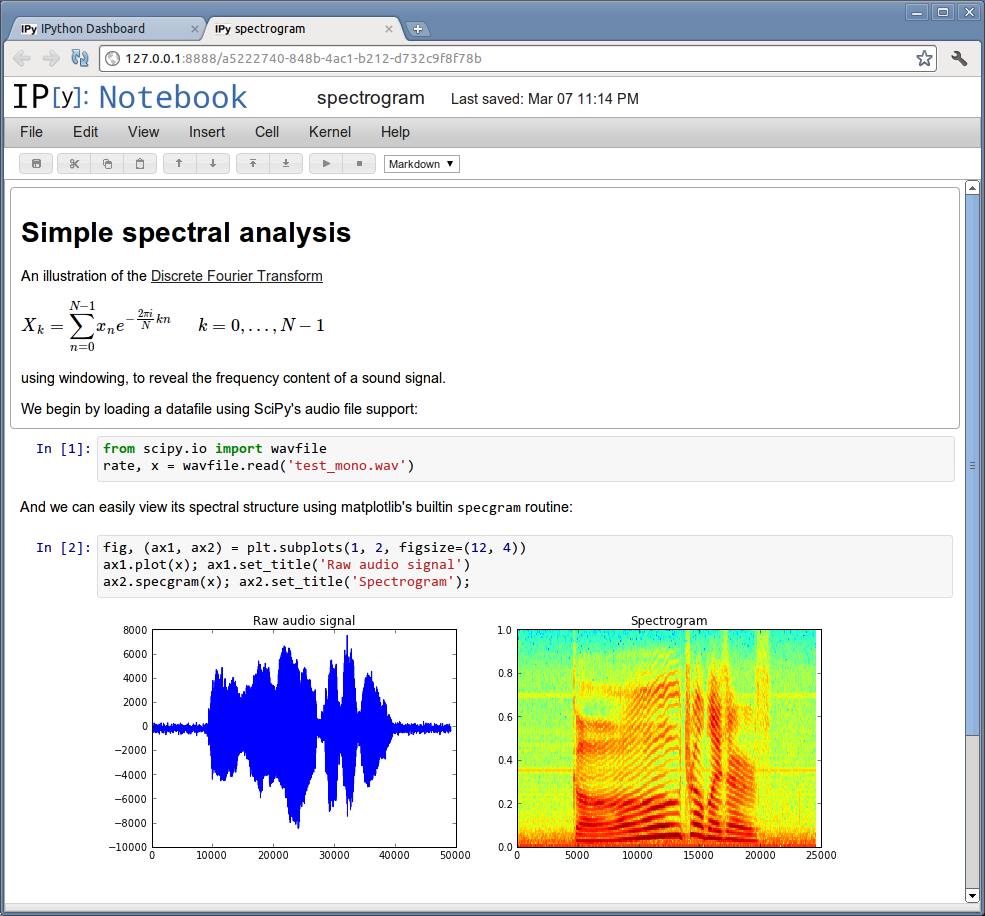
\includegraphics[width=3.2in]{fig/ipython-notebook-specgram.png}\par
  \end{centering}

  \caption{\label{fig:IPython-notebook}The web-based IPython Notebook combines
    explanatory text, mathematics, multimedia, code and the results from
    executing the code.}
\end{figure}

The driving idea behind the IPython Notebook is to enable researchers to move
fluidly between all the phases of the research life-cycle we described earlier.
If the environment where they conduct their exploratory research can also
support all subsequent stages of this cycle, and does so while smoothly
integrating with the version control and process practices we've previously
discussed, the likelihood that a final published result will be reproducible
increases significantly.  The Notebook system is designed around two central
ideas: (a) an openly specified protocol to control an interactive computational
engine, and (b) an equally open format to record these interactions between the
user and the computational engine, including the results produced by the
computations.

Before diving into the specifics of these two ideas, we note that the above
design is independent of the Python language: while IPython started its life as
a Python-specific project, the vision of the Notebook system is
language-agnostic.  First, while working in Python, users can mark entire code
blocks for execution via a separate language by using a special syntax on the
block's first line: a user can for example start a block \texttt{\%\%R},
\texttt{\%\%bash} or \texttt{\%\%ruby} and IPython will execute the entire
block with the respective system.  Second, an \emph{entire notebook} can be
executed in a different language if a remote engine (referred to as a
\emph{kernel}) exists that implements the interaction protocol.  As of this
writing, prototype kernels have been written in Ruby, JavaScript, and R, and
their development continues.

The IPython architecture provides a way to capture, version control, re-execute
and convert into other output formats, any computational session.  Notebooks
can be shared with colleagues in their native form for re-execution or
converted into HTML, \LaTeX, or PDF formats for reading and dissemination.  They
can be used in slideshow mode to give presentations that remain connected to a
live computation and can be exported into plain scripts for traditional
execution outside of the IPython framework.

The IPython protocol consists of messages in JSON (JavaScript Object Notation)
format that encode all actions that an interactive user can request of a
computational kernel, such as executing code, transferring data or sending
results, among many others.  While this protocol is implemented in IPython,
third-parties can independently implement it and provide new kernels that will
be able to interact with the notebook interface and clients.  The notebook file
format is a simple JSON data structure that contains a series of one or more
``worksheets'', each of which is a list of cells.  A cell can contain either
text or code, and code cells can also have the output corresponding to the
execution.  All sub-structures in the notebook format (the entire notebook, the
worksheets and the individual cells) have attached flexible metadata
containers; this metadata can be used by post-processing tools.  The file
format stores the communication protocol's payloads unmodified, so it can be
thought of as a structured and filtered log (since the user chooses what to
keep while working interactively) of the computation.  

The IPython project has taken elements pioneered by the Mathematica and Sage
notebooks and created a generic protocol and file format to control and record
literate computing sessions in any programming language.  This was a deliberate
choice in contrast to the literate programming approach: by providing a tool
that operates close to the live workflow of research computing (in contrast to
the batch-processing mode encouraged by classic literate programming tools),
the resulting documents are immediately reproducible sessions that can be
published in their own right or as companion materials to a more traditional
manuscript.  Given how IPython also includes support for parallel computing,
which we haven't discussed here in detail in the interest of conciseness, the
system provides an end-to-end environment for the creation of reproducible
research.

The real-world possibilities this offers were demonstrated during a
collaboration in 2012 between the IPython team, a microbiology team led by Rob
Knight from the University of Colorado and Greg Caporaso from the University of
Northern Arizona, and Justin Riley from MIT who created the StarCluster system
\mref{SC} for deployment and control of parallel resources on Amazon's EC2
cloud platform.  As part of an NIH-funded workshop to explore the future of
genomics data analysis in the cloud, this combined team collaborated on
creating a fully parallelized analysis comparing the predictive behavior of
different sizes and locations of gene sequence reads when reconstructing
phylogenetic trees.  The microbiologists had developed a serial prototype of
this idea using their Qiime libraries \mref{qiime}, but a large-scale analysis
with a full dataset would require roughly a month of CPU time on a single
workstation.  By locating the IPython Notebook server on Amazon cloud
instances, the entire team was able to log into a single instance and by
editing the code directly in the cloud, in a single day turn this prototype
into a set of production notebooks that would execute the analysis in parallel
using multiple Amazon servers.  Once the parallel was tested, it became evident
that there was not only an interesting example of using cloud technologies for
rapid development of research ideas but also a biologically relevant finding;
within a week the team had completed a more extensive run using 24 hours of
execution on 32 nodes and submitted a manuscript for publication \cite{RWM+12}.
This paper is now accompanied by all of the IPython notebooks that enable any
reader to fully reproduce our analysis, change parameters and question our
assumptions, without having to re-implement absolutely anything or be hampered
by lack of access to the code and data.  We have made available not only the
final notebooks, but also the Amazon Virtual Machine Images (data files that
represent a virtual computer on Amazon's cloud platform), so that the entire
analysis can literally be re-executed under identical conditions by anyone with
an Amazon account.

This example, anecdotal as it may be, indicates there is validity in the vision
we propose here: that by providing tools that encompass the entire cycle of
research, from exploration to large-scale parallel production and publication,
we can provide the scientific community with results that are immediately
accessible to others and reproducible, seeding the continued evolution of the
research process.

The IPython project also has developed tools that make it very easy to share
and disseminate content created as notebooks in a variety of forms.  The
Notebook Viewer hosted at \url{http://nbviewer.org} is a system that can render
\emph{any} publicly available IPython notebook as a web page.  This enables
users to share notebooks with others by simply putting them online and
pointing them to the rendered webpage, without the readers having to install
anything on their own systems.  And the same technology that powers the
notebook viewer service can also generate HTML files suitable for inclusion in
other websites, in particular, blogs.  Since a lot of rapid technical
communication is happening today on the Internet via blogs, this is an
important aspect of linking reproducible research to the rapid feedback cycle
of web-based discussion.  With a single command, a user can convert a notebook
file into HTML ready for posting to a blog, and this is already being used by
scientists to write both short technical posts and also more complex
materials: Jose Unpingco, a researcher with the US Department of Defense, is
currently working on a book titled \emph{Python for Signal Processing}, and
this book is available during writing as a GitHub
repository\footnote{\url{https://github.com/unpingco/Python-for-Signal-Processing}}.
This repository contains a series of IPython notebooks so that readers can
directly execute the code in the book, and they are also being published as a
series of blog posts as they become available, at
\url{http://python-for-signal-processing.blogspot.com}, so readers can comment
and discuss with the author throughout the process of book development, but
they can do so based directly on the actual code that creates all the examples
in the book.

The signal processing book is, to our knowledge, the first example of a full
book being written as a collection of executable IPython notebooks, but this
follows a tradition created by Mathematica, whose documentation is itself a
collection of executable Notebooks.  Furthermore, in recent years Rob Beezer,
from the University of Puget Sound, has developed popular Introductory Linear
Algebra book \mref{proper citation book is here:
  http://linear.ups.edu/html/fcla.html} that is based on the Sage system and
also combines the mathematics and text with code that can be directly executed
and modified by the readers.  It seems clear to us that this ability to ``close
the loop'' between what the authors had on their screens and what their readers
can execute themselves is an important element of the movement towards
reproducibility in research.

As a concrete implementation of the ideas of reproducible research using the
tools we've described in this chapter, during the ongoing process of research
itself, we can point to work being carried by a collaboration where one of us
(FP) is a member, on novel ways to model the mathematical structure of the
signal generated by MRI devices in the imaging of water diffusion in the
brain.  This work, as yet unpublished, is being developed as an open repository
on GitHub\footnote{\url{https://github.com/fperez/spheredwi}} where all code
for our research is posted during writing, all computational experiments are
created as IPython notebooks, and submitted manuscripts are created directly
from the code and notebooks (along with additional narrative written by hand).
This is an experiment we are conducting precisely with the intent of showing
that it is viable to conduct research in an open and reproducible way, with all
history of the code and manuscripts being held in publicly visible repositories
that anyone can download and replicate even prior to publication. 

We close this section by noting that the above tools are also playing a role in
the last stage of the cycle we outlined earlier, education.  We will increase
our chance that the next generation of scientists adopts improved
reproducibility practices if we educate them with the same tools that we use
for everyday research, and a couple of modern efforts that aim to bring
improved computational literacy to scientific research have adopted the IPython
notebook.  Software Carpentry\footnote{\url{http://software-carpentry.org}} is
a project funded by the Alfred P. Sloan Foundation and led by Greg Wilson at
the Mozilla Foundation whose motto is Richard Feynman's famous ``What I cannot
create, I do not understand.''  They produce, with rigorous follow-up and
assessment, workshops aimed at working scientists (typically graduate students
and postdocs, but always open to broad audiences) and whose purpose is to
instill in them a collection of skills and best practices for effectively using
computing as a daily research tool.  The Software Carpentry workshops cover
topics ranging from the basics of the Unix shell to version control, Makefile
automation of processes and basics of scientific Python including data analysis
and visualization.  They have recently adopted the IPython Notebook as the base
system for teaching the scientific Python parts of their curricula, and provide
the IPython team with direct feedback on its strengths and weaknesses as an
educational tool.  In a similar vein, Josh Bloom from the astronomy department
at UC Berkeley has led, for a number of years, a 3-day workshops on the use of
Python as a tool for scientific
computing\footnote{\url{http://pythonbootcamp.info}}.  These are open to the
entire campus community and followed by an optional for-credit seminar where
students learn more advanced skills for using Python as a research tool.
F. Pérez and other members of the IPython team at UC Berkeley regularly lecture
in the bootcamp and courses, where the notebook is the means for delivery of
course materials and interactive lecturing.  While we have identified a number
of weaknesses and areas for improvement, we have also found this environment to
be markedly superior to all previous tools we had used in the past for teaching
in similar contexts.

In summary, IPython embodies the main ideas we've woven into our discussion: it
was born out of the interplay between everyday scientific research and open
source software development, and it tries to be a natural part of the entire
research cycle in order to make it more fluid, efficient and reproducible.


\section{Conclusion}\label{conclusion}


As we seek to learn how the open source practice can inform our scientific
work, we must recognize that the ideal of scientific reproducibility
is by necessity a reality of shades. We can see a gradation that goes
from a pure mathematical result whose proof should be accessible to
any person skilled in the necessary specialty, to one-of-a-kind experiments
such as the Large Hadron Collider or the Hubble Space Telescope, that
can not be reproduced in any realistic sense. At each point in this
spectrum, however, we can always find ways to improve our confidence
in the results: whether we re-analyze the same unique datasets with
independently developed packages run by separate groups or we re-acquire
partial sampling of critical data multiple times, we should never
completely renounce the ideals of reproducibility because of practical
difficulties.

Similarly, in computational research we also have certain areas where
complete reproducibility is more challenging than others. Some projects
require computations carried on the largest supercomputers on the
planet, and these are expensive resources that can not be arbitrarily
allocated for repeated executions of the same problem. Others may
require access to enormous datasets that can not easily be transferred
to the desktop of any researcher wishing to re-execute an analysis.
But again, alternatives exist: it should be possible to validate scaled
versions of the largest problems run independently, against scaled
specimens created on the supercomputers for this purpose, and
sub-sampled datasets can be used to collect at least validation statistics
that may be informative of the trust we place on the published analysis.

%\begin{itemize}
%\item Levels of reproducibility: replication, validation, reproduction,
%new construction.
%\item Conditions: clarity, transparency and trace-ability, predictability
%(which requires automation), communicability
%\end{itemize}
%
%While the mechanical reproduction of computational results is not a
%panacea in itself; the rigor, openness, culture of validation, collaboration and
%other aspects of science must become a routine part of our computational practices.

\ldots

This is a large and complex problem that requires changing the educational
process for new scientists, the incentive models for promotions and
rewards, the publication system, and more.


Changing culture

%Open{*}: software, access (Elsevier), education, review.
%
%Internet: interactions for humans, code and data
%
%\begin{itemize}
%\item Open source software
%
%\begin{itemize}
%\item development akin to scientific culture
%\item viable alternatives to proprietary software
%\item tools and lessons for improving the scientific process: Github
%\end{itemize}
%
%\item Open access
%
%\begin{itemize}
%\item \url{thecostofknowledge.org}: Elsevier boycott
%\item FRPAA House hearing on March 29th.
%\end{itemize}
%
%\item Open review
%Ref \cite{10.3389/fncom.2012.00018}.
%
%\item Open education
%
%\begin{itemize}
%\item MIT Open Courseware, Khan Academy\ldots
%\item Stanford CS 221 in fall 2011: \textasciitilde{}160,000 students.
%\item Spring 2012:
%
%\begin{itemize}
%\item Sebastian Thrun leaves Stanford: Udacity.
%\item Stanford: Coursera.
%\end{itemize}
%\item MITx, TED-Ed\ldots
%\end{itemize}
%\end{itemize}

Incentive models

%Science has become computational, but the incentive models of science
%are single-mindedly focused on paper-oriented publications that completely
%ignore the computational process. Papers are accepted 
%
%What role should journals play?
%
%\begin{itemize}
%\item Journals should mandate that upon paper \emph{approval} (but before
%actual publication and with said publication being conditioned on
%the author meeting this last condition), authors must expose their
%version control system to the public, and that the publicly available
%version can faithfully reproduce (within the limitations discussed
%above) the published results. This public version then becomes available
%for the scientific community not only for download, but also as a
%starting point for further contribution and development.
%
%\item supplemental material
%
%\item peer review
%
%\item new BioMed Central journal, Open Research Computation
%
% \item ongoing thematic series in Source Code for Biology and Medicine.
%\cite{neylon2012changing}
%
%\end{itemize}
%
%How will all this impact scientists?
%
%\begin{itemize}
%
%\item funding
%\item academic merit review
%
%\end{itemize}

Education and training

%\paragraph{ {\bf Workshops}}
%
%\begin{itemize}
%
%\item Software carpentry
%
%\ldots basic training
%
%\item Python
%
%\ldots use of git
%
%\end{itemize}
%
%\paragraph{ {\bf Courses}}
%
%\begin{itemize}
%
%\item Josh
%
%\item Randy
%
%\item Titus
%
%\end{itemize}
%
%
\section*{Acknowledgments}
We would like to thank \ldots
%\begin{itemize}
%\item members of the scientific Python community
%\item scientist from various labs
%\item Brian Granger
%\item John Hunter
%\item reviewers
%\end{itemize}

\bibliographystyle{plain}
\bibliography{ipython}

\end{document}
